\newpage
\section{Resultados y Conclusión} \label{sec:conclusion}

En la figura~\ref{fig:escena_final} podemos observar un render con todos los objetos y
estructuras mencionadas en este trabajo.

\begin{figure}[H]
    \centering
    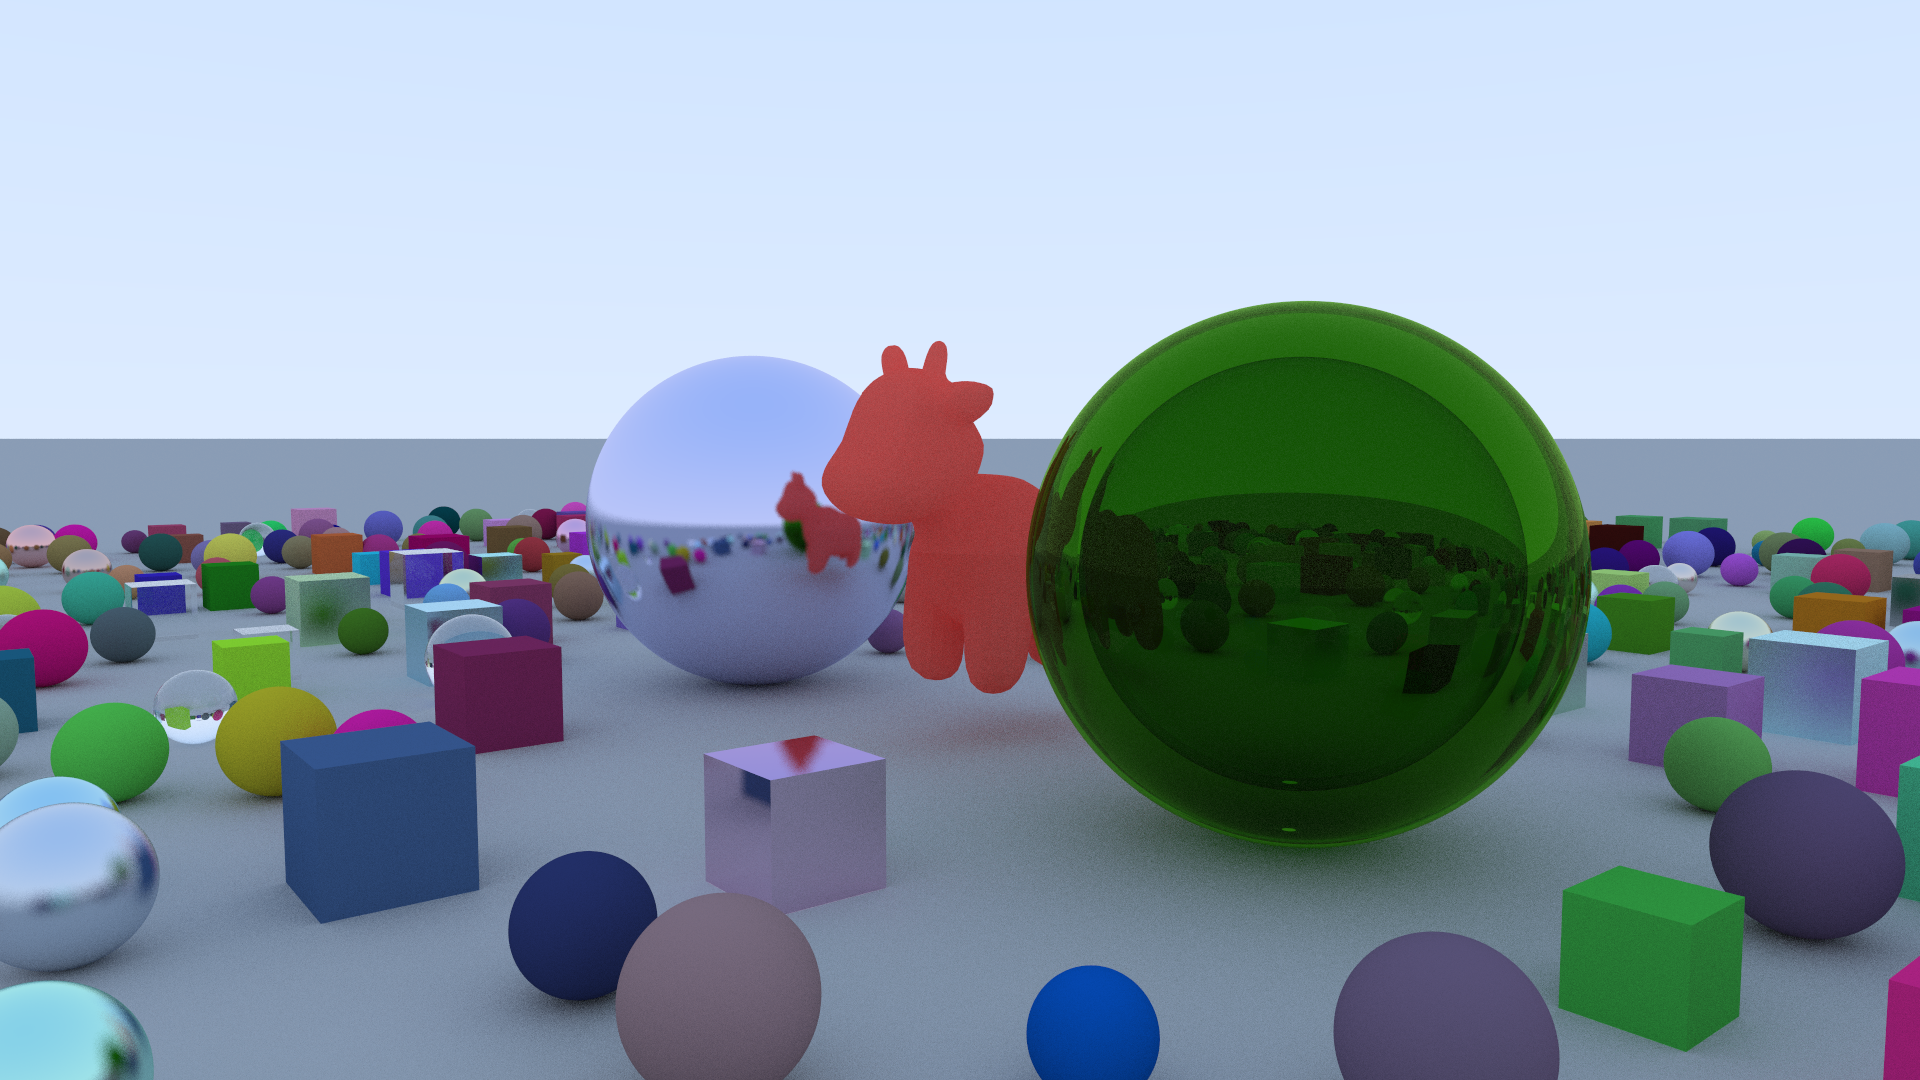
\includegraphics[width=.9\textwidth]{imgs/escena_final}
    \caption{Render de una malla de triángulos.}
    \label{fig:escena_final}
\end{figure}

Luego de ver en detalle dos técnicas de renderizado, una basada en \textit{object-order
rendering} (rasterización), y otra en \textit{image-order rendering} (ray tracing), las
diferencias son claras.

La rasterización cuenta con algoritmos que al día de hoy han sido optimizados a tal punto que
existe todo un pipeline dentro de la mayoría de las tarjetas gráficas.
Es necesario conocer este pipeline y la librería correspondiente para interactuar con el mismo, pero
su optimización resulta en renders de buena calidad en muy poco tiempo.

Por otro lado, los algoritmos de ray tracing suelen ser más intuitivos en cuanto a la idea
general y su implementación, y no requieren (en principio) de conocimientos de ninguna librería.
Si bien en la actualidad surgen nuevas tarjetas gráficas que incluyen unidades para realizar la
intersección de los rayos de manera optimizada, la realidad es que sin estos recursos el ray
tracing resulta lento en comparación a la rasterización.
Sin embargo, la calidad de las imágenes resultantes son claramente superiores y más realistas.

El futuro del ray tracing y su aplicación tanto en videojuegos como en producciones audiovisuales
resulta muy prometedor.
Las nuevas tarjetas gráficas capaces de realizar ray tracing en tiempo real permitirán que esta
rama de la computación gráfica avance a pasos agigantados y que la calidad del
contenido multimedia que producimos y consumimos crezca de manera acorde.